%!TEX root = ../../main.tex

\subsection{Ventilstyring Grænsefladebeskrivelse}

Ventilstyring er en grænseflade til systemet, modulet omsætter digital styring fra PSoC'en til analog aktuation i mangetventilen der kontrollerer vandtilførsel, udledning, samt dosering ved karret. 
Modulet tager, som input, et digitalt signal 0-5V. Dette omsættes til analog styring af ventilen. 
Derudover tilføres kontrolkredsen 12V som forsyningsspænding. fig.\ref{screenshot:tabel1},s.\pageref{screenshot:tabel1}

\begin{figure}[H]
	\centering
	\includegraphics[scale=0.6]{../Projektdokumentation/Systemarkitektur/Graenseflader/Screenshots/tabel1}
	\caption{Grænsefladebeskrivelse: Ventilstyring}
	\label{screenshot:tabel1}
\end{figure}


\subsection{Doseringspumpe Grænsefladebeskrivelse}

Doseringspumpen er ligeledes en grænseflade til systemet, modulet omsætter et digital PWM-signal fra PSoC'en til en procentvis styring af doseringspumpen så den kan kører i flere etaper. Modulet tager, som input, et digitalt PWM-signal 0-5V. Dette omsættes til analog styring i doseringspumpen. 
Derudover tilføres kontrolkredsen 12V som forsyningsspænding. fig.\ref{screenshot:tabel2},s.\pageref{screenshot:tabel2}  

\begin{figure}[H]
	\centering
	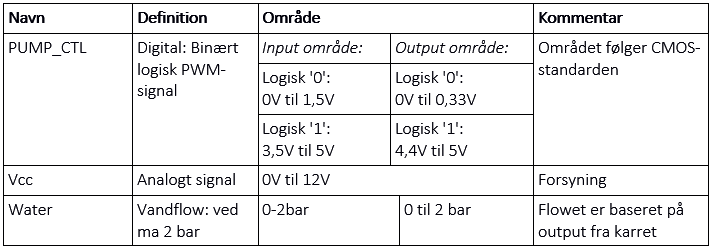
\includegraphics[scale=0.6]{../Projektdokumentation/Systemarkitektur/Graenseflader/Screenshots/tabel2_Pumpe}
	\caption{Grænsefladebeskrivelse: Doseringspumpe}
	\label{screenshot:tabel2}
\end{figure}


\subsection{Flowsensor Grænsefladebeskrivelse}
Flowsensor fungerer som grænseflade til systemet, modulet omsætter vandflow i sensoren til et digital PWM-signal der angiver hvor meget vand der flyder igennem sensoren. Modulet forsynes med +5V forsyning, samt GND, og afgiver PWM-signal 
Dette PWM omsættes via et eksternt counterkredsløb til at give logisk '1' ved hver 10. count. Dette trækker et interrupt i PSoC'programmet.fig.\ref{screenshot:tabel3},s.\pageref{screenshot:tabel3}

\begin{figure}[H]
	\centering
	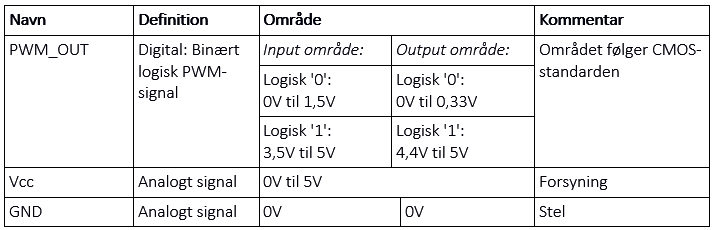
\includegraphics[scale=0.6]{../Projektdokumentation/Systemarkitektur/Graenseflader/Screenshots/tabel3_Flowsensor}
	\caption{Grænsefladebeskrivelse: Flowsensor}
	\label{screenshot:tabel3}
\end{figure}

\subsection{pH-probe Grænsefladebeskrivelse}
pH-proben måler pH-værdien i karet. Proben giver en analog spænding ud afhængig af pH-værdien i væsken. Karet omsætter denne værdi til en floating point. 

\begin{figure}[H]
	\centering
	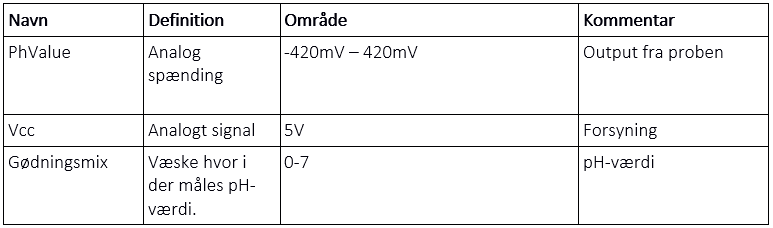
\includegraphics[scale=0.6]{../Projektdokumentation/Systemarkitektur/Graenseflader/Screenshots/tabel4_pH-probe.PNG}
	\caption{Grænsefladebeskrivelse: pH-probe}
	\label{screenshot:tabel4}
\end{figure}

\subsection{Jordfugt Grænsefladebeskrivelse}
Jordfugt måleren måler fugten i jorden. Her stikkes der nogle spyd ned i jorden, som giver en spænding ud afhængig af fugtigheden. PSoC'en omsætter denne spænding til en streng på I2C bussen.

\begin{figure}[H]
	\centering
	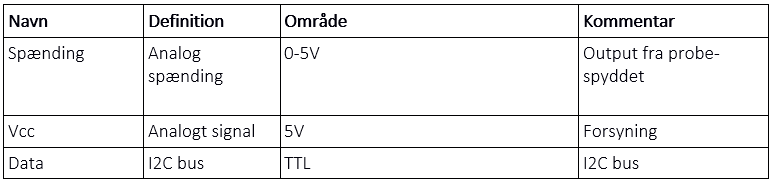
\includegraphics[scale=0.6]{../Projektdokumentation/Systemarkitektur/Graenseflader/Screenshots/tabel5_jordfugt.PNG}
	\caption{Grænsefladebeskrivelse: Jordfugt}
	\label{screenshot:tabel5}
\end{figure}

